\section{Spørgsmål 5}

\subsection{Fokuspunkter}

\begin{itemize}
	\item Hvad er normalisering og hvorfor bruges normalisering?
	\item Kom bla. ind på begrebet funktionelle afhængigheder.
	\item Samt redegør kort for normalformerne fra 1 til 4 Normalform (1..4NF)
\end{itemize}

\subsection{Litteratur}
\begin{itemize}
	
	\item Fra teori: Database Modeling and Design. Logical Design 5'th Ed.
	\begin{itemize}
		\item Kap. 6 (s. 109 - 130, ekstensivt s. 117 - 128).
	\end{itemize}
	
	\item Fra Database eLearning: \url{http://db.grussell.org/index.html}.
	\begin{itemize}
		\item Normalisation.
		\begin{itemize}
			\item Normalisation 0NF-3NF.
			\item Normalisation BCNF and Example.
		\end{itemize}
	\end{itemize}
	
	\item Fra wikipedia:
	\begin{itemize}
		\item \href{https://en.wikipedia.org/wiki/Database_normalization}{Database normalization}
		\begin{itemize}
			\item \url{http://en.wikipedia.org/wiki/Fourth_normal_form}
		\end{itemize}
	\end{itemize}
%	
%	\item Fra Agile Data Home Page:
%	\begin{itemize}
%		\item 
%	\end{itemize}
\end{itemize}

\newpage

% must
\subsection{Hvad er normalisering og hvorfor bruges normalisering?}\label{sec:normal}
Normalisering er den process der organiserer data i en database. Processen omfatter oprettelse af tabeller og etablering af relationer mellem tabellerne i henhold til et sæt regler, Normalformerne. Normalisering foretages for at minimere data redundancy. Normalisering prøver at opnå isolation af data, således at man kan Delete, Inserte og Update på en enkelt tabel, hvorpå ændringerne propageres gennem resten af databasen vha. fremmednøgler.

I en ikke normaliseret database kan man støde på disse propblemer:

\begin{itemize}
	\item \textbf{Update Anomaly} - Samme information findes i flere records. Dette kan føre til inconsistancy i forbindelse med Update.
	\item \textbf{Insertion Anomaly} - Når information ikke kan gemmes. Eksempel på databasen nedenfor hvor Course Code ikke kan være NULL
	\item \textbf{Deletion Anomaly} - Når en tabel indeholder mere end én slags information. Eksemplet med fakultet og kurser, viser hvorledes Dr. Giddens forsvinder hvis man fjerner hans record.	
\end{itemize}

\begin{figure}[H]
	\centering
	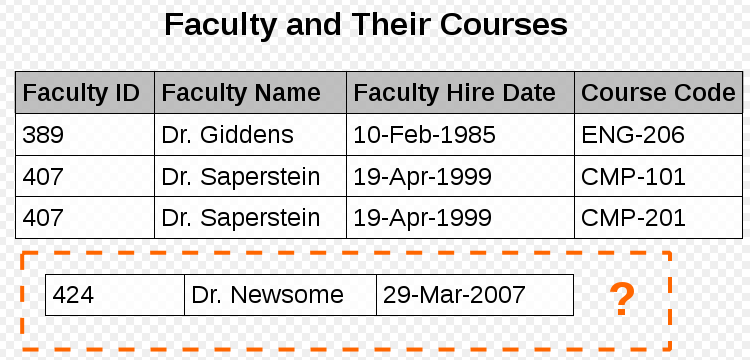
\includegraphics[width=0.7\linewidth]{figs/spm5/insertionAnomaly.PNG}
	\caption{Eksempel på insertion anomaly}
	\label{fig:insertionAnomaly}
\end{figure}

For at undgå disse anomalies bruges Normalformer.

% must
\subsection{Kom bla. ind på begrebet funktionelle afhængigheder}
En funktionel afhængighed (FD) er en afhængighed mellem felter i en tabel.
Et eksempel på en FD kunne være Postnummer og by, hvor postnummer determininerer By, altså har vi \textbf{postnummer $\rightarrow$ by}. På samme måde med Navn og CPR hvor \textbf{CPR $\rightarrow$ Navn}

\textbf{X$\rightarrow$Y}
\subsubsection{Transistive afhængigheder}
En afhængighed hvor tre eller flere felter indgår.
\textbf{X$\rightarrow$Y$\rightarrow$Z}


% must
\subsection{Samt redegør kort for normalformerne fra 1 til 4 Normalform (1..4NF)}

\subsubsection{1. Normalform}
Den mest basale normalform. Følgende gør sig gældende:

\begin{itemize}
	\item 1NF overholdes kun hvis hver kolonne i en tabel kun kan holde \textbf{én} værdi. 
\end{itemize}

Med andre ord må der ikke, i et \textit{telefonnummer} felt skrives flere numre. 

F.eks ville \textit{45659885,78856532} ikke overholde reglen.

%\begin{figure}[H]
%	\centering
%	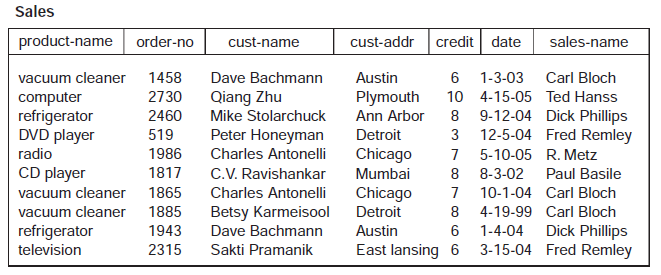
\includegraphics[width=0.8\linewidth]{figs/spm5/notNormalizedTable.PNG}
%	\caption{Sales Tabellen overholder 1NF, da ingen attributter indeholder mere en 1 værdi.}
%	\label{fig:notNormalizedTable}
%\end{figure}

Tabeller i 1NF findes der ofte duplikerede data, samt dårlig performance, og Update integritet.\todo{Woot? Forstod intet. Lyder meget overfladisk?}
	
\subsubsection{2. Normalform}
Er kun opfyldt hvis nedenstående punkter gør sig gældende. Se figur~\ref{fig:not2NF} for en tabel der ikke opfylder 2NF.
	
\begin{figure}[H]
	\centering
	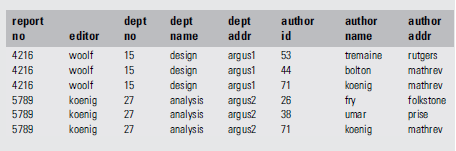
\includegraphics[width=0.8\linewidth]{figs/spm5/not2NF.PNG}
	\caption{1NF er opfyldt, ikke 2NF}
	\label{fig:not2NF}
\end{figure}
	
	
\begin{itemize}
	\item 1NF er opfyldt.
	\item Alle non-key attributter er fuldt ud afhængige af primærnøglen. Enten transistativ afhængig eller direkte.\todo{Ikke forstået?}
\end{itemize}
	
I en tabel hvis primærnøgle er sammensat\todo{Censor spørger: Kan du pege på den sammensatte primærnøgle?}, skal de felter som kun er afhængige af en del af disse, flyttes over i en tabel for sig, sammen med en kopi af den primærnøgle som de er afhængige af.

På figur~\ref{fig:2NF} ses tabellen som nu opfylder 2NF. 

\begin{figure}[H]
	\centering
	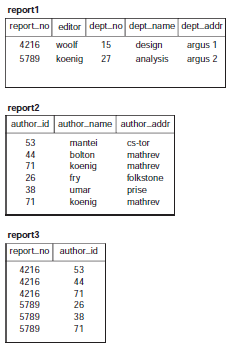
\includegraphics[width=0.5\linewidth]{figs/spm5/2NF.PNG}
	\caption{Sales tabellen opfylder nu 2NF}
	\label{fig:2NF}
\end{figure}
	
\subsubsection{3. Normalform} 
Er kun opfyldt hvis følgende gør sig gældende.

\begin{itemize}
	\item Transitative afhængigheder fjernes.
	\item En tabel der indeholder felter som er indbyrdes afhængige\todo{Find eksemple} og ikke er en del af primærnøglen, skal disse flyttes over i en ny tabel med en kopi af primærnøglen som de er afhængige af.
\end{itemize}
	
\paragraph{NF3,5 - Boyce-Codd normalformen} i de fleste tilfælde er BNCF opfyldt i 3NF. Hvis BNCF ikke opfyldes er følgende gældende:
	
\begin{itemize}
	\item Der er mere end en kandidatnøgle i relationen, og mindst en af dem er en kompositnøgle.\todo{Woot?}
\end{itemize}
	
\subsubsection{4. Normalform}
Er next level af Boyce-Codd normalformen (også kaldet 3.5NF). Denne normalform handler ikke om FD'er men derimod om \textbf{Multivalued dependancies}. Der må altså ikke være repeterende felter.\\

Eksempel med tabellen Person(CPR,Uddannelse,Hobby). Hvis samme person har flere hobbyer, X og flere uddanneler, Y vil der altså komme XY tupler for at dække alle muligheder. Løsningen er at dele tabellen op i to: 

\textbf{Uddannelse(CPR, Uddannelse)} og \textbf{Fritid(CPR, Hobby)}. Her er der kun brug for X+Y tupler i to tabeller.

